\chapter{Background}
\section{Parallel Programming Languages for HPC}
High Performance Computing (HPC) refers to computation performed on supercomputers. 
Supercomputers generally have more and faster cores than personal computers. They are normally networked together with fast interconnect to allow for high data throughput, and are used for highly numerical scientific programs.
To fully leverage the potential of these supercomputers' many computing cores, programmers use parallel computing techniques, in programming languages which, when compiled to programs, run as fast as possible on the hardware. Parallel computing within HPC usually refers to decomposing a problem into seperate tasks, and then solving those tasks at the same time, on different pieces of hardware.

The three main languages used in HPC are Fortran, C and C++. They are all well established within the field, as shown by table~\ref{tab:langs}, which shows the proportion of compute time taken up by these languages on ARCHER, (Advanced Research Computing High End Resource), one of the UK's primary academic research supercomputers.
Whilst Fortran takes up the majority of compute time on ARCHER, this dissertation will focus on C and C++, as they are more comparable to Rust (their similarities are discussed further in the sections~\ref{sec:c} and~\ref{sec:rust}).

\begin{table}[h]
  \centering
  \begin{tabular}{|c|c|}
    \hline
    Language & \textbf{ARCHER} \\
    \hline
    Fortran & 69.3\% \\
    \hline
    C++ & 7.4\% \\
    \hline
    C & 6.3\% \\
    \hline
    Unidentified & 19.4\% \\
    \hline
  \end{tabular}
  \caption{Breakdown of CPU usage by programming language on ARCHER~\cite{Turner2015}}
  \label{tab:langs}
\end{table}

There are two paradigms to parallel computing: message passing parallelism and shared memory parallelism. In message passing parallelism, processes work on private data, and share data by sending and receiving messages. This form of parallelism is very scalable, and can run on geographically distributed heteregenous nodes~\cite{SETI}. Examples of message passing parallelism include the MPI (message passing interface) standard, and Go's channels.

Shared memory parallelism, by comparison, has processes that share access to a region of memory. Whilst programs using shared memory parallelism can run on multiple nodes through technologies like PGAS (Partitioned Global Address Space), these nodes are still normally required to be homogenous. Shared memory parallelism is most effective when it runs on a single node with many processing cores. This effectiveness is seen in GPU programming, which extensively uses shared memory parallelism.
Shared memory parallelism is a fast way to write and run programs, but there are difficulties inherent in implementing this technique in languages like C and C++ that are not memory safe. In the next section, I will discuss these difficulties.

\section{C and C++}\label{sec:c}
The C programming language was developed in 1972, as a `system implementation language'~\cite{Ritchie:1993}. Its first purpose was to program the UNIX operating systems and the utilities which were fundamental to its use, like \texttt{cat} and \texttt{rm}. Since that point, the C programming language has always been associated with low level computing. In this case, low level computing means computing which is able to be compiled to very efficient machine code, and gives the programmer fine grained memory management. Low level computing is close to the model presented by the hardware, with very few abstractions.

Today, the Linux kernel, which provides the foundation for the operating systems used on the vast majority of the world's supercomputers, is 96\% written in C~\cite{LinuxKernel}. Many of the programs that are run on these supercomputers are written in C~\cite{fftw, ffs, foam}

Despite C's success, only seven years after it was first developed, Bjarne Stroustrup began working on an extended version of C, which was to become C++. In 1985, the first commercial edition of C++ was released~\cite{DandE}. Two of C++'s most notable extensions to C are the introduction of classes, to allow for object oriented programming, and templates, which allow for generic programming. C++ also uses a stronger type system than C, which prevents bugs caused by implicit conversion.

Like C, the design of C++ focused on system programming~\cite{CplusEssence}, and like C, it has become a common language of choice for developing HPC codes~\cite{foam, tensorflow, lammps, gromacs}, a fact which is helped by the close similarity of the two languages. Many C programs are valid C++ programs. C and C++ are also considered two of the languages which, when compiled, run fastest.

The speed of C and C++ is one of their most celebrated design features. However, there are other, less positive consequences of the design of these two languages, which require programmers to use them with care. This dissertation is principally concerned with the memory safety issues of C and C++, which can cause programs to crash, or return incorrect data.

Listing~\ref{lst:use-free} demonstrates one of C and C++'s memory pitfalls, known as~{\em use after free}. The code is syntacically valid C and C++ which compiles. Use after free occurs when a program attempts to use a section of memory after it has been released back to the operating system.
The freeing of \texttt{array} here means that the contents of it cannot be guaranteed when it is printed, resulting in undefined behaviour.

\begin{code}
\begin{minted}{c}
#include <stdio.h>
#include <stdlib.h>

int main(){
    int* array = (int*) malloc(sizeof(int)*10);
    for (int i=0; i<10; i++){
        array[i] = i;
    }
    free(array);
    printf("%d\n", array[1]);
    return 1;
}
\end{minted}
\captionof{listing}{C and C++: Use after free}
\label{lst:use-free}
\end{code}

In larger programs, this can lead to calculations being made using incorrect data, which has been overwritten by the operating system, or another thread from the same program. Defensive techniques such as `Resource Acquisition Is Initialisation' (RAII) can be used to prevent such problems, but ultimately rely on the programmer to implement them.
Other common sequential memory pitfalls in C and C++ are:

\begin{itemize}
    \item \textbf{Double Free:} Attempting to free memory which has already been freed can lead to undefined behaviour.
    \item \textbf{Heap Exhaustion:} The program tries to allocate more memory than the amount available. This can be the result of a memory leak, when data is not always freed after being allocated.
    \item \textbf{Buffer Overrun:} Attempting to access the $n^{th}$ element of an array which is only of length $n$. This can lead to the reading incorrect data, or accidentally corrupting other memory within the same program.
    \item \textbf{Data Race:} This type of non-deterministic bug occurs when two or more threads need to update a variable, but the outcome of this update depends on the timing of the threads accessing the variable. An example of a data race is given in listing~\ref{lst:omp-eg}.
\end{itemize}

Whilst it is possible to write memory safe code with memory unsafe languages, it is hard to do so. It is impossible to know how exactly many bugs exist in HPC codes, and to know how many of those are caused by memory safety issues.
As an indication, we can take data from Microsoft, which shows that 70\% of their Common Vulnerabilities and Exposures (CVEs) are caused by memory safety issues~\cite{MicroBugs}. There is no good estimate of the amount of memory safety errors that exist in C or C++ HPC programs, but if we take the Microsoft data to be indicative of general error sources, then the lack of memory safety in C and C++ should be a cause of concern for HPC programmers.

\subsection{OpenMP}
The first specification for the OpenMP (Open Multi-Processing) Fortran, C and C++ language extension Application Program Interface (API) was released in October 1998. Its aim was to `allow users to create and manage parallel programs while permitting portability'~\cite{OpenMPSpec}. It acts as an extension to the C and C++ language specifications, leaving responsibility for implementing it to compiler writers, just as with C and C++. New specifications of OpenMP are periodically released, and it is now recognised as a cornerstone of HPC, as can be seen from the large number of people who sit on the its Architecture Review Board from diverse institutions and industry bodies~\cite{OpenMPARB}.

OpenMP's parallelism model is based around shared memory parallelism. This is done to reflect the reality of the multi-core hardware which are used in HPC\@. Multi-core processors share memory with each other, and each core can access any memory address on that node.  

An example OpenMP program is shown in listing~\ref{lst:omp-eg}. It is syntacically valid C and C++ which compiles. A key feature of OpenMP are its \texttt{\#pragma omp} statements, which issue parallelism related directives to the compiler. 
One of OpenMP's core strengths is its succinct abstractions to the underlying threading API, irrespective of the platform it is running on.
Here, the \texttt{\#pragma omp parallel} statement signifies the part of the code to be parallelised, and importantly, does not do so at the cost of obscuring the program's serial intent.
The example parallelises the for loop, and sets the number of threads through the \texttt{OMP\_NUM\_THREADS} environment variable. In this program, the variable \texttt{a} is set to zero, and it is then incremented in the for loop.

\begin{code}
\begin{minted}{c}
#include <omp.h>
#include <stdio.h>
int main(){
    int a = 0;
    #pragma omp parallel for
    for (int i=0; i<10; i++){
        a++;
    }
    printf("%d\n", a);
    return 0;
}
\end{minted}
\captionof{listing}{C and C++: OpenMP data race causes incorrect result}
\label{lst:omp-eg}
\end{code}

However, the output of this program is non-deterministic, as it includes a data race condition. The type of data race here is read modify write, where each thread reads the variable, adds one, and then writes back to the original memory address.
The problem occurs when two threads try to read the variable at the same time, e.g. they both read a value of $1$. Both threads then add $1$ to the value they have read, and write back to the orginal memory address. 
Both threads perform $1+1$, get a value of $2$, and write that value. The correct behaviour is for the first thread perfoms $1+1=2$, and the second thread performs $2+1=3$.

To solve this problem, a \texttt{\#pragma omp atomic} statement must be inserted at in the line above \texttt{a++}. As with the other memory errors mentioned earlier however, these mistakes are not always found before using a program.

\section{Rust}\label{sec:rust}
The Rust programming language was launched by the Mozilla Foundation in 2011~\cite{FutureTense}. Rust's design was stated to aim towards being a `static, structured, concurrent, large-systems language'~\cite{pServo}. Like C and C++, Rust's early design aims included the goal of becoming a systems language.
Rust also uses the LLVM backend, just like the C and C++ compiler clang~\cite{rustClang}.
Rust even has C-like structs, and shares behaviours between those structs through composition with traits, not with inheritence, like C++.

Rust's initial design ideas mainly diverge from C and C++ in its aims to provide the programmer with memory safety. Two ideas, ownership and immutability are used to achieve this improvement. 

Ownership is one of Rust's more unique features. It `allows Rust to be completely memory-safe'~\cite{NomOwner}, and works by using the compiler's borrow checker to ensure that Rust's ownership model is satisfied by a given program before compiling it.

In listing~\ref{lst:rust-free} we present a Rust program that does not satisfy the ownership model, and therefore does not compile. The first line of the main function heap allocates memory to a vector of 10 elements, and gives each element a value of four. This vector is labelled \texttt{vector}. It is created using a macro, which is similar to functions in Rust, except that they can take a variable number of arguments, formatted in different ways, like with semi-colons.

\begin{code}
\begin{minted}{rust}
fn main(){
    let vector = vec![4;10];
    drop(vector);
    println!("{}", vector[2]);
}
\end{minted}
\captionof{listing}{Rust: Use after free results in a compile time error}
\label{lst:rust-free}
\end{code}

The \texttt{drop()} function is then called on the vector, which is similar to \texttt{free()}. \texttt{drop()} is automatically called on values when they go out of scope. It is more accurate to think of \texttt{drop()} as something akin to C++'s destructors, but both those and this function do, at their core, release memory back to the operating system. However, attempting to use a variable after it has been dropped is illegal in Rust, resulting in the error message below:

\begin{code}
\begin{minted}{bash}
error[E0382]: borrow of moved value: 'array'
 --> src/main.rs:6:20
  |
2 |     let vector = vec![4;10];
  |         ----- move occurs because 'array' has type 'std::vec::Vec<i32>',
  which does not implement the 'Copy' trait
3 |     drop(vector);
  |          ----- value moved here
...
6 |     println!("{}", vector[2]);
  |                    ^^^^^ value borrowed here after move

error: aborting due to previous error
\end{minted}
\captionof{listing}{Rust Compiler: Use after free error log shows the lines at which the error was made}
\label{lst:rust-borrow-move}
\end{code}

This is Rust's borrow checker telling the programmer that the program does not follow the ownership model. When the value of \texttt{vector} is dropped, in the Rust ownership model, the ownership of \texttt{vector} is moved into the drop function, and is not returned.
When the program later tries to use (borrow) the variable, it is therefore unable to, as Rust only allows for values to have one owner at a time.


Allowing values to only have one owner at a time is worked around by functions borrowing mutable or immutable references to those variables. For example, if a function needs to mutate a vector, it will need to specify that type in its function arguments, e.g. \texttt{v: \&mut Vec<i32>}, where \texttt{v} is of the type of a borrowed mutable reference to a vector containing 32 bit integers.
This requirement also highlights how Rust's borrow checker is re-enforced by a strong type system, which requires the function parameter to be of a certain type, and immutability by default, which makes it explicit which functions will change values that are passed to them.

Memory safety is further improved in Rust by the absence of null pointers through the use of optional values. If a function may return something or nothing, it returns an \texttt{Option<T>}, which can either be \texttt{Some(v)} where \texttt{v} is a value of type \texttt{T}, or \texttt{None}. Pattern matching can be used to succinctly unwrap these variables.

Rust also makes the promise that it is free of data races, with certain caveats. Data races are defined as:
\begin{itemize}
    \item `two or more threads concurrently accessing a location of memory
    \item one of them is a write
    \item one of them is unsynchronized'
\end{itemize}
\begin{flushright}
--- The Rustonomicon: Data Races and Race Conditions~\cite{NomRace}
\end{flushright}

and are only absent from {\em safe Rust}. This does not mean that Rust prevents programmers from creating deadlock situations entirely, only that a certain subsection of data races are prevented, and only in safe Rust.
Unsafe Rust exists as another language within Rust, delimited within \texttt{unsafe} blocks. It exists because there a limits to such a safe Rust which do not accurately reflect the underlying hardware on which it runs. Safe Rust protects the programmer from type safety and memory safety issues, whilst unsafe Rust allows the programmer unfettered access to the underlying hardware, with all the risks that entails.
However, unsafe not seen as being the `\textit{true} Rust Programming Language'~\cite{NomSafe}, and therefore this dissertation will only examine safe Rust. 
Unlike C and C++, Rust comes with a build tool and dependency manager, Cargo, which wraps around the Rust compiler. Cargo allows users to specify a program's dependencies, which are automatically downloaded and integrated into that program from external repositories. In Rust, these dependencies are called {\em crates}.

Traits are used by Rust to define behaviour for generic data types. A class can implement many traits which are implemented by other classes. In this way, a classes behaviour is composed, and not inherited like in C++.

Some work has been done to investigate the applicability of Rust to HPC~\cite{bioinformatics, blanco2016}, but it is still not seen as a standard within the HPC community. As such, I will gain technical support from the Rust community through the official subreddit and community discord channels when I encounter a problem particular to Rust.

\subsection{Rayon}\label{sec:back-rayon}
Rayon is the one of the most popular crates for parallelism in Rust, and features heavily in the Rust cookbook~\cite{RustCookPara}. In a fashion similar to OpenMP, it abstracts complicated underlying threading technologies. Unlike OpenMP, Rayon concentrates on parallel iterators, and like Rust promises data race freedom.

Rayon's parallel iterators are conceptually descended from Rust's sequential iterators. An iterator is a function which provides access to the elements of a collection, so that an operation can be performed on a set of those elements. In Rust, iterators are data collections which implement the \texttt{Iterator} trait, which provides access to the current item, and a \texttt{next()} function, which returns an optional value.
An example of a sequential iterator is shown in listing~\ref{lst:rust-seq-iter}, where a vector of 5 elements, each with value 2, are first each multiplied by five in the \texttt{map()} function, using an anonymous function. In Rust, these are called closures. The \texttt{fold()} function then returns the product of all the elements in the mapped collection, which is 10000. The first argument of fold provides the identity value for the fold, which is used to begin the operation.

Rayon's parallel iterators work in a similar way to Rust's sequential iterators, except that they give sections of the iterable collection to separate threads to calculate. The parallel iterator methods also have slightly different syntax, as demonstrated by listing~\ref{lst:rust-par-iter}. This listing produces the same result as~\ref{lst:rust-seq-iter}, but the \texttt{fold()} is different.

\noindent\begin{minipage}{.49\textwidth}
\begin{code}
\begin{minted}{rust}
fn main(){
  let v = vec![2;5];
  let s = v.iter()
           .map(|x| x * 5)
           .fold(1, |acc, x| acc * x);
  println!("{}", s);
}
\end{minted}
\captionof{listing}{Rust: sequential iterator}
\label{lst:rust-seq-iter}
\end{code}
\end{minipage}\hfill
\begin{minipage}{.49\textwidth}
\begin{code}
\begin{minted}[fontsize=\scriptsize]{rust}
extern crate rayon;
use rayon::prelude::*;

fn main(){
  let v = vec![2;5];
  let s = v.par_iter()
           .fold(|| 5, |acc, x| acc * x)
           .reduce(|| 1, |x, y| x * y);
  println!("{}", s);
}
\end{minted}
\captionof{listing}{Rayon: parallel iterator}
\label{lst:rust-par-iter}
\label{lst:iters-a}
\end{code}
\end{minipage}

The first argument to the parallel \texttt{fold()} is an identity closure, which generates the identity value. This is done so that the different threads can have their own copy of the identity value. The output of the fold is different too, as each thread performs a fold on its section, and therefore does not return a single value. A parallel reduction is called on the resulting collection, which delivers the product of all the values left in the collection.\todo{see rupe's note}
In this way, the fold reduce pattern is `roughly equivalent to map reduce'~\cite{rayonFold} in effect. It is also noteworthy that \texttt{par\_iter()} uses a number of threads set by the environment variable \texttt{RAYON\_NUM\_THREADS}, which is similar to OpenMP\@.

Iterators are safer than for loops because they prevent threads trying to access data beyond array boundaries, without a performance cost. However, they do lack flexibility compared to for loops. From within a for loop, the programmer can access the $i^{th}$ element of the collection they are iterating over, or the $i-1^{th}$ element, if they choose to through simple index arithmetic. I will investigate the costs and the benefit of this trade off in when porting programs to Rust, in section~\ref{sec:meth}.

\section{Mini-apps and Kernels}
In computing a {\em kernel} is often used to describe a part of a larger program that is responisble for much of that programs execution time. Within the context of this dissertation however, I will use kernel to describe the whole of a very small program, which is itself representative of a common HPC task. In this way, my usage of kernels is similar to how mini-apps have been used in research.

Mini-apps are a well established method of assessing new programming languages or techniques within HPC~\cite{Mallinson:2014, Slaughter:2015, martineau2017arch}. A mini-app is a small program which reproduces some functionality of a common HPC use case. Often, the program will be implemented using one particular technology, and then ported to another technology. The performance of the two mini-apps will then be tested, to see which technology is better suited to the particular problem represented by that mini-app. Such an approach gives quantitative data which provides a strong indication for the performance of a technology in a full implementation of an application. 
\section{Roofline}
The Roofline model~\cite{williams2009roofline} shows how a program's performance is constrained by the processor it runs on. The model plots operational intensity against attainable work. 

Operational intensity is measured in floating point operations, or Flops, per byte.
This metric usefully relates the amount of work done to the amount of data that it is done to. If more work is done to less data, the operational intensity will be higher, and if less work is done to more data, the operational intensity will be lower.


\begin{figure}[h]
\centering
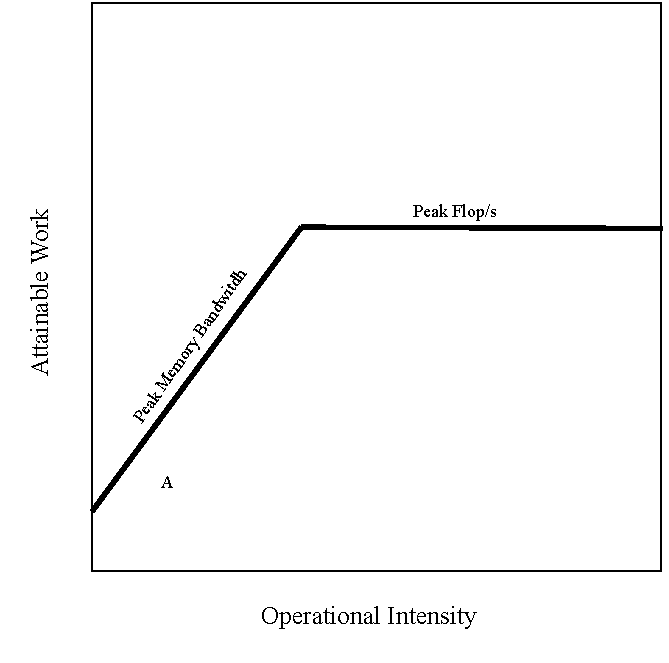
\includegraphics[width=.66\linewidth]{figs/roofline.pdf}
\caption{Theoretical Roofline}\label{fig:roof-eg}
\end{figure}

Attainable work is measured work is measured in Flops per second, and shows the frequency that work is done at. If more work is done in less time, the Flops per second will be higher, and if less work is done in more time, the Flops per second will be lower.

Figure~\ref{fig:roof-eg} shows a theoretical example of the a Roofline model, where boundaries for peak memory bandwidth and peak Flop/s have been added. Theses boundaries have the advantage of showing how close programs come to meeting the limitationts of the hardware they are running on, and give the programmer insights into potential bottlenecks which their program is suffering from. 
For example, if the programmer wishes for program A in figure~\ref{fig:roof-eg} to achieve a greater amount of Flops, they must also increase the operational intensity of their program so that A is no longer bounded by the peak memory bandwidth.

In a similar way, I will use the Roofline model to assess how different implementations of my selected kernels are able to effectively and efficiently use the hardware they run on. The Roofline model should illustrate where the different implementations of the kernel's bottlenecks lie, which in turn will give me good insight into the applicabilty of Rust to HPC.
